% !TeX program = xelatex
\documentclass{vilgym}

% For math
\usepackage{mathtools}
\usepackage{amsfonts}

% For graphs
\usepackage{graphicx}

% For wrapping text
\usepackage{wrapfig}

\usepackage{float}

% General info
\title{Kunsti genereerimine teksti põhjal}
\author{Karl-Joan Alesma, III MF}
\instructor{õp Malle Eglit}
\date{2020}

% Define expected value operator
\DeclareMathOperator{\EX}{\mathbb{E}}
\DeclareMathOperator{\loss}{\mathcal{L}}
\DeclarePairedDelimiter{\norm}{\lVert}{\rVert}

\DeclareNameAlias{sortname}{family-given}
\addbibresource{viited.bib}
%\DeclareNameAlias{sortname}{family-given}

\usepackage{xpatch}

% Remove parenthesis around year
\xpatchbibmacro{date+extradate}{%
  \printtext[parens]%
}{%
  \setunit*{\space}%
  \printtext%
}{}{}

\begin{document}
	\maketitle
	\tableofcontents

	%\unsection{Definitsioonid}
	%\begin{description}
	%\let\originalitem\item
	%\renewcommand*{\item}[1][]{\originalitem[#1]\label{def:#1}}

	%\item{GAN} ing.k. \textit{generative adversarial network}
	%\end{description}

	\newcommand*{\seefig}[1]{(\hyperref[fig:#1]{vt~joonis~\ref{fig:#1}})}
	\newcommand*{\inglk}[1]{(\textit{ingl. k. #1})}

	\unsection{Sissejuhatus}
	Sügavõpe \inglk{Deep Learning} on meetodite kogu, mis võimaldab õpetada arvutile, kuidas lahendada erinevaid probleeme. Antud valdkond on eksisteerinud juba alatest 1940. aastatest (küll aga teise nime all), kuid on alles hiljuti saanud populaarseks. Kiire areng ja edasiminek on peamiselt tingitud arvutusressurside kasvust ning järjest suurenevast andmete hulgast. Need kaks asjaolu on võimaldanud treenida sügavamaid, keerulisemaid ning täpsemaid mudeleid. \parencite{deeplearningbook}	 

	Üks uus mudel, mis on sügavõppe kiire arengu jooksul tekkinud, on GAN ehk generatiivne adverstiivne võrk. Antud võrku on võimalik treenida jäljendama erinevaid andmete distributsioone. Kasutades treenimise käigus õpitud esindusvorme, suudab see võrk genereerida uut materjali, mis on sarnane treenimisel kasutatud andmetega. \parencite{gan}

	Uurimistöö eesmärk on luua mudel, kasutades GANe, mis on võimeline genereerima kunsti teksti põhjal. Andes mudelile sisendiks kirjelduse, milline peab olema loodava kunstiteose sisu ja mis stiilis, genereerib mudel teose, mida tegelikkuses ei eksisteerigi. Lisaks saab autor selle protsessi käigus kinnitada ja laiendada oma teadmisi sügavõppest.

	Kuna puuduvad digitaalsed andmekogud, kus oleksid olemas teoste kirjeldused (nt \enquote{Pildil on mees, kes raiub puid, ning tema selja taga on karu.}), ei ole võimalik treenida ühte GANi, mis suudaks teisendada sisu kirjelduse kunstiteoseks. Selleks kasutab autor kahte GANi --- esimene GAN teisendab sisu kirjelduse vastavaks pildiks (sisu\textrightarrow pilt), mis antakse järgmisele GANile, mis muudab loodud pildi kunstiteoseks soovitud stiilis (pilt\textrightarrow kunst).

	Hüpotees on, et mudel, mis on treenitud genereerima ainult ühte kindlat objekti sisaldavaid teoseid (ehk mudel suudab luua teoseid, kus on näiteks ainult linnud), loob realistlikumaid teoseid kui mudel, mis on treenitud genereerima mitmeid erinevaid objekte sisaldavaid teoseid (ehk mudel suudab luua teoseid, kus on näiteks majad, metsad või muu selline).

	Töö alguses annab autor ülevaate varasematest töödest selles valdkonnas ning tutvustab loogikat, mille põhjal on mudel kokkupandud. Seejärel vaadeldakse erinevaid mudeleid, millele järgneb eksperimentaalne osa, kus analüüsitakse ning hinnatakse erinevate mudelite sooritust. 
	
	\section{Varasemad tööd}

	Uue materjali genereerimine on keeruline probleem. Kogu sügavõppe ajaloo vältel on diskrimineerivad mudelid (mudelid, mis eristavad sisu) saavutanud paremaid tulemusi kui generatiivsed mudelid (mudelid, mis loovad sisu). Hiljuti on aga see muutunud GANide tekkega \parencite{gan}. GANid on saavutanud märkimisväärseid tulemusi pildi \parencite{biggan} ja video genereerimises \parencite{dvdgan} ning saanud hakkama ka pildi resolutsiooni suurendamise ehk superresolutsiooniga \parencite{srgan}. GANide edu põhjuseks on kahe närvivõrgu omavaheline võistlus, mille tulemusel genereeritud materjali kvaliteet paraneb ideaalis seni, kuni on eristamatu päris materjalist. GANi tööpõhimõtet tutvustatakse järgmises peatükis.

	Pildi genereerimine tekstist on huvitav probleem, mille arengus on hoogu andnud GANide kasutuselevõtt. Reed jt kasutasid sisendist sõltuvat GANi \inglk{conditional GAN}, millele anti sisendiks tekstist närvivõrguga eraldatud sisu, et genereerida 64x64 suurusega pilte \parencite{reed}. Nende järgmine töö kasutas peale tekstisisendi ka objekti asukohta, mis parandas loodud piltide kvaliteeti \parencite{reed2}. 

	Zhang jt kasutasid kahte GANi, et genereerida parema resolutsiooniga pilte. Esimene GAN genereerib ligikaudse visandi, millele teine GAN lisab detaile ning suurendab resolutsiooni \parencite{stackgan}. Antud lähenemine on lihtsam kui pildi genereerimine ühe GANiga. Nende järgmine töö kasutas kolme GANi, mis olid ühendatud jadamisi, et genereerida järjest suurema resolutsiooniga pilte. \parencite{stackgan2}.

	Xu jt mudel AttnGAN kasutab samuti 3 GANist koosnevat struktuuri, aga millele on juurde lisatud tähelepanumehhanism \parencite{attngan}. Tähelepanu võimaldab mudelil joonistada erinevaid alamregioone, keskendudes sõnadele, mis on antud piirkonna jaoks kõige olulisemad. Autor kasutab mudelis Xu jt mudelit komponendina, mis muudab sisu kirjelduse pildiks (sisu\textrightarrow pilt), kuna antud mudeli tulemused on teiste omadest paremad. 

	Selleks, et muuta tavaline pilt kunstiteoseks, on kaks erinevat võimalust --- stiili ülekanne või CycleGAN. Stiili ülekanne võtab sisendiks sisupildi ja stiilipildi ning proovib seejärel genereerida pildi, mille sisu on sarnane sisupildiga ja mille stiil on sarnane stiilipildiga \parencite{styletransfer}.
	Selleks kasutatakse varem treenitud pildidklassifitseerija erinevaid kihte, et mõõta kahe pildi vahelist sisu ja stiili sarnasust. 

	CycleGAN võimaldab treenida see-eest GANi, mis teisendab sisendpildi ühest hulgast teise. Näiteks mustvalge pildi värviliseks, sebra hobuseks või antud juhul pildi kunstiteoseks. Treenimise käigus kasutatakse põhimõtet, et kui muuta mustvalge pilt värviliseks, siis saadud värvilise pildi teisendamisel mustvalgeks, peaks jõudma tagasi algse musta pildini. \parencite{cyclegan}

	Kui võrrelda CycleGANi ja stiiliülekannet, siis stiiliülekande puudujäägiks on tema võime ainult teisendada ühe pildi stiil teisele pildile, samas kui CycleGAN suudab teisendada terve piltide kollektsiooni stiili soovitud pildile. Zhu jt on ka leidnud, et Gatys jt meetodil ei õnnestu tihti luua fotorealistlikke pilte \parencite{cyclegan}. Autor kasutab mudelis CycleGANi komponendina, mis muudab pildi soovitud stiiliga teoseks (pilt\textrightarrow kunst), kuna antud mudel suudab kanda üle terve kollektsiooni stiili ning luua tõepärasemaid pilte.

	Leidub varasemaid töid, kus on kasutatud GANi, et genereerida kunsti, näiteks ArtGAN \parencite{artgan}, GANGough \parencite{gangough} ja CAN \parencite{can}. Need mudelid kasutavad valdavalt ühte tingivat GANi ($ G(\boldsymbol{z}|\boldsymbol{\theta}) $, $ \boldsymbol{z} $ on müravektor ja $ \boldsymbol{\theta} $ on stiilivektor), mis võimaldab genereerida erinevas stiili ja sisuga teoseid. Sellise viisi puhul saab muuta loodavat sisu muutes vektorit $ \boldsymbol{\theta} $, mis muudab peamiselt loodava teose stiili ja seega loodavat sisu, aga ei võimalda täpselt määrata loodava teose sisu. 

	Kasutades antud töö autori ideed, on teoreetiliselt võimalik kontrollida teose sisu ja stiili ning mille puhul on ka samast sisendtekstist genereeritud teosed erinevad. Kuna puuduvad andmed kunstiteoste ja nende kirjelduste vahel, ei saa genereerida kunsti, mille sisu saab kirjeldusega määrata, ainult ühe GANiga. Seega koosneb autori mudel kahest GANist --- AttnGANist (sisu\textrightarrow pilt) ja CycleGANist (pilt\textrightarrow kunst). %, mida edaspidi nimetan text2art-ganiks.


	%  \section{Mudel}
	\section{Tehnilised detailid}
	Eelmises osas anti põgus ülevaade erinevadest mudelitest. Selles osas kirjeldatakse põhjalikumalt, kuidas töötab GAN, AttnGAN ja CycleGAN.

	\subsection{GAN}
	\spacing{1.39}
	Generatiivne adversatiivne võrk ehk GAN \inglk{generative adversarial network} on sügavõppe mudel, mis koosneb kahest neuronvõrgust --- üks on diskrimineerija \inglk{discriminator} ja teine on generaator \inglk{generator}.  Generaatori ülesandeks on luua sisu, mis on sarnane kasutuselolevate andmete jaotusega. Diskrimineerija ülesandeks on määrata, kas talle näidatud sisu on võetud päris andmete hulgast või on loodud generaatori poolt.
	
	Generaatoril ja diskrimineerijal on vastastikused ülesanded --- diskrimineerija proovib minimeerida viga, mis tehakse sisu klassifitseerimise käigus (kas on võetud päris andmete hulgast või loodud generaatori poolt), ja generaator proovib maksimeerida viga, mida diskrimineerija teeb klassifikatsiooni käigus. Kokkuvõtvalt mängivad need kaks võrku omavahel minimaksmängu \inglk{minimax}, mida võib võrrelda vägikaikaveoga. Lõpuks jõutakse Nashi tasakaalu \inglk{Nash equilibrium}, kus osalejatel ei ole enam midagi võita oma strateegia muutmisega \parencite{gametheory}. Ideaalis on sel juhul diskriminaatori poolt väljastatud tõenäosus sõltumata sisendist $ 1/2 $.

	Ilustavalt võib mõelda generaatorist kui võltsijate meeskonnast, kes proovivad luua võltsraha ja kasutada seda ilma jäljeta. Diskrimineerija aga käitub kui politsei, proovides tuvastada kas tegu on võltsinguga. Alguses on võltsijatel võltsingud kehvad ning politseil on raskusi tuvastusega, aga aja jooksul muutuvad osapooled paremaks omavahelise võistluse tõttu, kuni hetkeni, mil võltsingud pole enam eristatavad päris valuutast.

	Treenimisprotsessi saab võtta kokku järgmise funktsiooniga:
	\begin{equation} \label{eq:gan}
		\operatorname*{min}_G \operatorname*{max}_D \loss_{GAN}(D,G) = \EX_{\boldsymbol{x}\sim p_{andmed}(\boldsymbol{x})}[\log D(\boldsymbol{x})] + \EX_{\boldsymbol{z}\sim p_{\boldsymbol{z}}(\boldsymbol{z})}[\log(1-D(G(\boldsymbol{z})))]
	\end{equation}
	kus $ \boldsymbol{z} $ on müravektor, mis on võetud distributsioonist $ p_{\boldsymbol{z}} $ (nt ühtlane- või normaaljaotus), $ \boldsymbol{x} $ on päris pilt, mis on võetud distributsioonist $ p_{andmed} $, $ G $ on generaatorfunktsioon ja $ D $ on diskrimineerimisfunktsioon. Treenides $ G $ ja $ D $ vaheldumisi, treenitakse GANi looma sisu, mis sarnaneb treenimisel kasutatud andmete distributsiooniga. \parencite{gan}
	\spacing{1.4}

	\subsection{AttnGAN}

	AttnGAN on mudel, mis suudab genereerida pilti sisendiks antud teksti põhjal. Kui anda mudelile sisendiks pildi kirjeldus \enquote{sellel väikesel linnul on punane pea ja kõhualune, valged tiivad ning lühike nokk}, siis mudel suudab antud sisendi põhjal luua kirjeldusele vastava pildi \seefig{attngan}.
	
	\begin{wrapfigure}{l}{0.55\textwidth}
		\includegraphics[width=0.53\textwidth]{images/attngan.png}
		\caption{Tekstist genereeritud pildid; vasakult poolt minnes suureneb resolutsioon}
		\label{fig:attngan}
	\end{wrapfigure}

	Mudeli sisemuses on 3 GAN, mis on üksteisega jadamisi ühendatud. Iga GAN genereerib järjest suuremaid pilte --- esimene genereerib 64x64, teine 128x128 ja kolmas 256x256 \seefig{attngan}. Antud struktuur võimaldab eespool olevatel GANidel genereerida ligikaudseid kujusid ja värve ning hilisematel GANidel juba täpsemaid detaile. Teoorias on võimalik lisada veel GANe üksteise otsa, mis võimaldaks genereerida kõrgema resolutsiooniga pilte, aga selle tulemusena suureneks treenimiseks kuluv aeg (on vaja teha rohkem arvutusi) ning võib juhtuda, et mudel variseb lihtsamini kokku (kõik sisendpildid langevad kokku ühe väljundpildiga).

	AttnGANis on tekstikodeerija, mis eraldab sisendtekstist sõna- ja lausetunnused. Eraldatud lausetunnusvektor ning müravektor antakse sisendiks esimesele GANile, mis genereerib esimese pildi. Esimese ja teise GANi vahel on tähelepanumehhanism, mis kasutab just genereeritud pilti ning eraldatud sõnatunnuseid, et leida sõna-konteksti vektor, mis määrab ära kui oluline mingi sõna teatud regiooni kujundamisel on (lihtsamalt öeldes pööratakse iga sõna puhul tähelepanu neile pildi osadele, mida see sõna kirjeldab). Esialgne pilt ning sõna-konteksti vektor kombineeritakse ning antakse seejärel sisendiks teisele GANile, mis genereerib järgmise pildi. Analoogne mehhanism on ka teise ja kolmanda GANi vahel.

	Treenimise jaoks kasutatakse peale klassikalise GANi funktsiooni ka mudelit, mille nimi on sügava tähelepanu multimodaalne sarnasusmudel ehk lühemalt DAMSM \inglk{Deep Attentional Multimodal Similarity Model}. Antud mudel leiab, kui sarnased on omavahel sisendtekst ning genereeritud pilt. Kuna selle mehhanismi tööpõhimõte on keeruline, siis saab sellega lähemalt tutvuda Xu jt töös. \parencite{attngan}

	\subsection{CycleGAN}
	\begin{figure}
		\centering
			\includegraphics[width=\linewidth]{images/cyclegan_est.png}
			\caption{CycleGAN suudab teisendada pilte erinevate domeenide vahel \parencite{cyclegan}}
			\label{fig:cyclegan}
	\end{figure}

	CycleGAN on GAN, mis lahendab pildi pildiks teisendamise probleemi, kus soovitakse õppida seost sisendpildi ning väljundpildi vahele. Näiteks teisendades mustvalget pilti värviliseks pildiks või teisendades õhufotot kaardiks \seefig{cyclegan}. Varasemad meetodid on ainult töötanud olukordades, kus on olemas pildipaarid. Nende kogumine on aga kallis ning keeruline, mille tõttu on valmis andmekogumid pildipaaridest väikesed. CycleGANiga on võimalik õppida seos sisend- ning väljundpildi vahel isegi olukordades, kus puudub andmekogum pildipaaridest. 

	Kui on antud sisend pildikogum $ X $ ja väljund pildikogum $ Y $, siis eesmärk on leida selline seos $ G: X \rightarrow Y $, et genereeritud pilt $ \hat{y} = G(x), x \in X $ oleks eristamatu pildist $ y \in Y $. Selleks kasutatakse vastast (diskrimineerijat) $ D $, mis on treenitud eristama $ y $-t $ \hat{y} $-st. 

	Sellise lähenemisega kerkivad esile teatud probleemid --- antud seos ei kindlusta, et $ x $ ja $ y $ oleksid paari seatud tähendusrikkal viisil, kuna on olemas lõpmatult palju seoseid $ G $, mis loovad sama jaotuse üle $ \hat{y} $. Peale selle leidsid töö autorid, et on raske optimeerida kasutades ainuüksi klassikalise GANi eesmärkfunktsiooni, kuna see võib viia mudeli kokkuvarisemiseni, kus kõik sisendpildid langevad kokku ühe väljundpildiga ning optimeerimine ei suuda parandada enam tulemust.

	Probleeme aitab lahendada põhimõte, et teisendus peab olema tsükliliselt järjepidev. Teisisõnu, kui tõlkida lause eesti keelest inglise keelde ning seejärel tagasi, siis peaks jõudma tagasi algse lauseni. Selle rakendamiseks on vaja kahte teisendust --- olgu esimene teisendus $ G\colon X \rightarrow Y $ ja teine teisendus $ F\colon Y \rightarrow X $, siis peaksid $ G $ ja $ F $ olema üksteise pöördfunktsioonid. Et seos oleks tsükliliselt järjepidev, lisandub klassikalise GANi eesmärgile eesmärk, mis motiveerib tsüklilist järjepidevust ($ F(G(x)) \approx x $ ja $ G(F(y)) \approx y $).
	\begin{equation}
		\loss_{cyc}(G,F) = \EX_{x\sim p_{andmed}(x)}[\norm{F(G(x)) - x}_1] + \EX_{y\sim p_{andmed}(y)}[\norm{G(F(y)) - y}_1]
	\end{equation}

	Töö autorid leidsid ka, et kui teisendada maastikumaale fotodeks, siis muutsid generaatorid $ G $ ja $ F $ tihti pildi tooni. Selleks toodi	juurde identiteet seos, mis hoiab generaatoreid pilte muutmast, kui pilt juba näeb välja nagu pilt, mida proovitakse saada.
	\begin{equation}
		\loss_{idt}(G,F) = \EX_{y\sim p_{andmed}(y)}[\norm{G(y) - y}_1] + \EX_{x\sim p_{andmed}(x)}[\norm{F(x) - x}_1]
	\end{equation}

	CycleGANi puhul on erinev ka GANi põhieesmärk:
	\begin{equation}
		\loss_{GAN}(G,D_Y, X, Y) = \EX_{y\sim p_{andmed}(y)}[\log D_Y(y)] + \EX_{x\sim p_{andmed}(x)}[\log(1-D_Y(G(x)))]
	\end{equation}
	
	Seega täiseesmärk on:
	\begin{equation} \label{eq:cyclegan}
		\begin{aligned}
			\loss(G, F, D_x, D_y) &= \loss_{GAN}(G, D_y, X, Y) + \loss_{GAN}(F, D_x, Y, X) \\
								  &+ \lambda_{cyc} \loss_{cyc}(G, F) + \lambda_{idt} \loss_{idt}(G, F)
		\end{aligned}
	\end{equation}
	kus $ D_y $ on $ G $ diskriminaator, mis proovib eristada $ G(x) $ ja $ y $, $ D_x $ on  $ F $ diskriminaator, mis proovib eristada $ F(y) $ ja $ x $, ning $ \lambda_{cyc} $ ja $ \lambda_{idt} $ on hüperparameetrid, mis vastavalt määravad, kui oluline on $ \loss_{cyc} $ ja $ \loss_{idt} $ täiseesmärgi juures. \parencite{cyclegan}

	\subsection{Mudel}
	Selle töö poolt väljapakutud mudel koosneb kahest komponendist --- AttnGANist, mis muudab sisendteksti pildiks, ning CycleGANist, mis muudab AttnGANi poolt loodud pildi kunstipäraseks. Lisaks sisendtekstile, määratakse ära, millisesse stiili CycleGAN pildi teisendab.

	AttnGAN ja CycleGAN mudelite jaoks kasutati vundamendina nende tööde autorite poolt kirjutatud koodi, et hoida kokku aega ning vältida vigade tekkimist koodis, ning mida muudeti seejärel vastavalt vajadusele, et sobituda kokku töö eesmärgiga.

	Et hoida kokku aega ning arvutiressursse, kasutas autor AttnGANi jaoks varem treenitud mudeleid, kuna AttnGAN ümbertreenimine ei oleks kuidagi parandanud väljapakutud mudeli sooritust.

	CycleGANi puhul tuli iga stiili jaoks ning parameetri muutmise korral treenida uus mudel. Kokku treeniti 10  mudelit, kus igat ühte treeniti ligikaudu 40 tundi RTX 2080 graafikakaardiga. Kahjuks jõudis autor treenida CycleGAN tegema ainult kahte erinevat stiiliteisendust, aga tulevikus on plaan lisada veel teisigi stiiliteisendusi. Treenimise käigus olid võrrandi number \ref{eq:cyclegan} parameetrite väärtused $ \lambda_{cyc} = 10 $ ja $ \lambda_{idt} = 0.5 $.

	Töö kood ning treenitud mudelid, mida on võimalik ka oma arvutis jooksutada, on kättesaadavad GitLabis \parencite{text2art-gan}.

	\section{Eksperimendid}
	Selles peatükis hinnatakse välja pakutud mudeli edukust realistliku kunsti loomisel ning selle sisu kooskõla sisendtekstiga.

	\subsection{Andmekogud}
	AttnGAN treenimiseks kasutati CUB \parencite{cub} ja COCO \parencite{srgan} andmekogusid. CUB on andmekogum lindudest, kus on $\approx$ 10 000 pilti, kus iga pildi kohta on 10 erinevat kirjeldust. COCO on laiahaardelisem andmekogum, kus on pilte loomadest, sõidukitest, toidust ning mitmetest muudest objektidest. Andmekogus on $\approx$ 80 000 pilti, kus iga pildi kohta on 5 erinevat kirjeldust.

	CycleGANi treenimiseks kasutati Wikiart'i andmekogumit \parencite{wikiart}. Tegu on andmekoguga, kus on $\approx$ 80 000 erinevat kunstiteost, millele on juurde lisatud stiil, žanr, autor jne. Selle asemel, et andmeid uuesti kogutud, kasutas autor Tan jt poolt varasemalt kokku korjatud Wikiart andmekogumit \parencite{artgan}. Treenimiseks kasutati kategooriaid abstraktne ekspressionism ja impressionism.

	\begin{figure}
		\includegraphics[width=\linewidth]{images/linnud.jpg}
		\caption{Vasakul on AttnGANi poolt genereeritud pilt (sisendtekst on piltide all) ning paremal rakentatud stiilid}
		\label{fig:cub}
	\end{figure}

	\subsection{CUB}
	Tulemustest on näha, et AttnGANil õnnestub üsna hästi luua realistlikke lindude kujutisi, mis vastavad ka teksti kirjeldusele, kuid on see-eest ka linde, millel on erinevaid moonutusi, nagu kaks pead või pole pead ega jalgu. CycleGANil õnnestub rakendada stiili genereeritud pildile üsna edukalt \seefig{cub} --- leidub pilte, mis näevad kunstiteoste moodi välja, aga leidub ka pilte, kus pole stiili rakendatud või stiili on hoopis rakendatud liiga jõuliselt, mille tõttu mõjub pilt häirivana.

	Autor katsetas ka $ \lambda_{idt} $ väärtuse muutmisega võrrandis \ref{eq:cyclegan} nii et $ \lambda_{idt} = 5 $. Valdavalt olid selle mudeli poolt loodud teosed pehmemate toonidega ning tekstuur oli ka sujuvam. Abstraktse stiili puhul oli näha rohkem eredamaid toone.

	Tulevikus tasub proovida veel teisigi lambda väärtusi, mis on 0.5 ja 5 vahel või neist hoopis suuremad.

	\subsection{COCO}

	\spacing{1.38}
	Sellel mudelil on raskusi realistlike kunstiteoste genereerimisega \seefig{coco}. Kuna andmekogu sisaldab pilte mitmetest erilaadi objektitest, on AttnGANil raskusi seose leidmisega teksti ja piltide vahel (pildid küll meenutavad teose kirjeldust, aga ei ole väga detailsed) ning ka CycleGANil on selle tõttu raskusi stiili ülekandmisega (valdavalt muudab CycleGAN natuke värvi ning tekstuuri). Mudeli tulemust võiks parandada pikem treenimine, aga raske on hinnata millisel määral.

	\begin{wrapfigure}{l}{0.37\textwidth}
		\includegraphics[width=0.35\textwidth]{images/distribution.png}
		\caption{Jaotuse erinevus: vasakul pool on sisend, mida CycleGAN saab treenimisel, ning paremal poole sisend, mida CycleGAN tegelikult saab; piltide all on sisendtekst}
		\label{fig:dist}
	\end{wrapfigure}

	Kuna AttnGANi poolt genereeritud pildid ei ole väga realistlikud, on selle tõttu erinev pildijaotus, mida kasutati \mbox{CycleGANi} treenimiseks (treenimisele kasutati päris pilte AttnGAN genereeritud piltide asemel, lootuses, et AttnGAN poolt genereeritud pildid on realistlikud ning et CycleGAN suudab üldistada neile), pildijaotusest, millele CycleGAN kannab stiili üle \seefig{dist}. Pildijaotuse lõhe vähendamiseks kasutati COCO testimisandmekogu 5000 erinevat kirjeldust, et genereerida 5000 uut pilti, mida kasutati seejärel CycleGANi treenimiseks.

	On näha, et selle meetodi tulemusel paranes stiiliülekande edukus pisut. Loodud pildid pole nii udused ning on näha rohkem toonimuutusi ja detaile. Mõlema meetodi edukus võib ka varieeruda juhuse tõttu.

	\begin{figure}[ht]
		\includegraphics[width=0.9\linewidth]{images/coco.png}
		\caption{Vasakul on AttnGANi poolt loodud pilt (sisendtekst on pildi all); vasakult teises tulbas on pildid, mille loomiseks kasutati CycleGANi, mis on treenitud päris piltidel; viimase kahe tulba puhul on CycleGAN treenitud AttnGANi poolt genereeritud piltidel}
		\label{fig:coco}
	\end{figure}
	Kuna genereeritud piltidel treenimine parandas mudeli edukust, hindas autor mudeli sooritust ka kui $ \lambda_{idt} = 5 $. Selle väärtuse muutmisel võis täheldada samasugust mõju, mida oli näha CUB andmekogu puhul. Värvitoonid muutusid pehmemaks ning tekstuur sujuvamaks. 
	\spacing{1.4}

	Sisendiks ei pea aga andma kirjeldusi, mis kirjeldaksid ainult olukordi. Mudelile võib anda ka sisendiks abstraktsemaid mõisteid, nagu armastus, kurjus ja õnnelikkus \seefig{abstract}. Selle tulemusel võivad tekkida väga huvitavad ja omapärased teosed. Sisendiks saab kasutada aga ainult selliseid sõnu, mida on kasutatud COCO andmekogus olukordade kirjeldamiseks ehk teisisõnu peab mudel olema neid sõnu varem näinud.

	\begin{figure}[ht]
		\includegraphics[width=\linewidth]{images/abstraktne.png}
		\caption{Genereeritud pildid, millele on antud sisendiks pildi all olev abstraktsem mõiste}
		\label{fig:abstract}
	\end{figure}
	\unsection{Kokkuvõte}
	Uurimistöö eesmärgiks oli luua mudel, mis oleks ise võimeline genereerima tekstist kunsti, sai täidetud. Peale selle leidis ka kinnitust hüpotees, et mudelid, mis genereerivad ainult ühte objekti sisaldavaid pilte, loovad realistlikumaid pilte. Seda selle tõttu, et andmekogust, mis sisaldab mitmeid objekte, on programmil raskem järeldusi teha.
	
	Üleüldise mudeli sooritusega võib jääda rahule --- kui genereerida suurem kogus pilte, siis nende hulgas leidub ka pilte, mis näevad välja nagu need oleks kunstniku poolt tehtud pildid. 

	Programm suudab luua ka üsna huvitavaid tulemusi kui anda sisendiks abstraktsemaid mõisteid, nagu viha, rõõm või armastus. Sisendiks saab kasutada aga ainult sõnu, mida on varem kasutatud andmekogus piltide kirjeldamiseks.
	
	Mudelite keerukuse tõttu, kulus nende treenimiseks palju aega (kokku 400h). Peale selle on vaja iga andmekogu ja hüperparameetri väärtuse muutmise korral treenida uus mudel. Nende põhjuste tõttu jõudis autor treenida mudelit tegema ainult kahte erinevat stiiliteisendust, aga tulevikus on plaan lisada juurde ka teisi teisendusi.

	Tööprotsessi käigus sai autor paremini aru, kuidas töötab GAN ning mis põhimõtted on võrrandi number ühe taga. Peale selle sai autor kogemust juurde koodi lugemisel ja selle kirjutamisel ning ka erinevate teadustööde läbi töötlemisel.

	\unsection{Summary}
    The main goal of this research paper was fulfilled --- build a model, that can generate art from text descriptions. In addition to this, the hypothesis, that models that are trained on a dataset, which contain only images of a single object, perform better compared to models trained on a multiobject dataset. This is due to the fact that a dataset which contains multiple objects are harder and more difficult for the model to generalize to.
    
    The overall performance of the model is adequate --- if one were to generate a large collection of pictures then it would most certainly contain images, that look like they were made by an artist.

    The model can also generate very interesting results if given more abstract words, for example, hatred, happiness or love. You can only use words for text descriptions that have been used to describe pictures in the datasets.

    Due to the complexity of the task, it took a tremendous amount of time to train each model (in total 400h). Furthermore, it is necessary to train a different model for each dataset and each change made to a hyperparameter. As a result the author only managed to train the model to make two different style transfers but there are plans to add more style transfers in the future.
    
    During the process, the author developed a better understanding of how a GAN works and what the intuition and thought process behind the equation number one is. The author also gained experience in reading and writing code as well as in the perusal of other people's research papers.
	% The bibliography
	\nocite{*} % List all entries, even when not cited
	\printbibliography[title={Kasutatud allikad}]

	\appendices
	\appendix{CUB}
	
	\begin{figure}[H]
		\includegraphics[width=0.8\linewidth]{images/lisa1.png}
		\caption{Iga stiil vasakpoolse tulba puhul $ \lambda_{idt} = 0.5 $ ja parempoolse tulba puhul $ \lambda_{idt} = 5 $}
		\label{fig:lisa1}
	\end{figure}

	\appendix{COCO}
	\begin{figure}[H]
		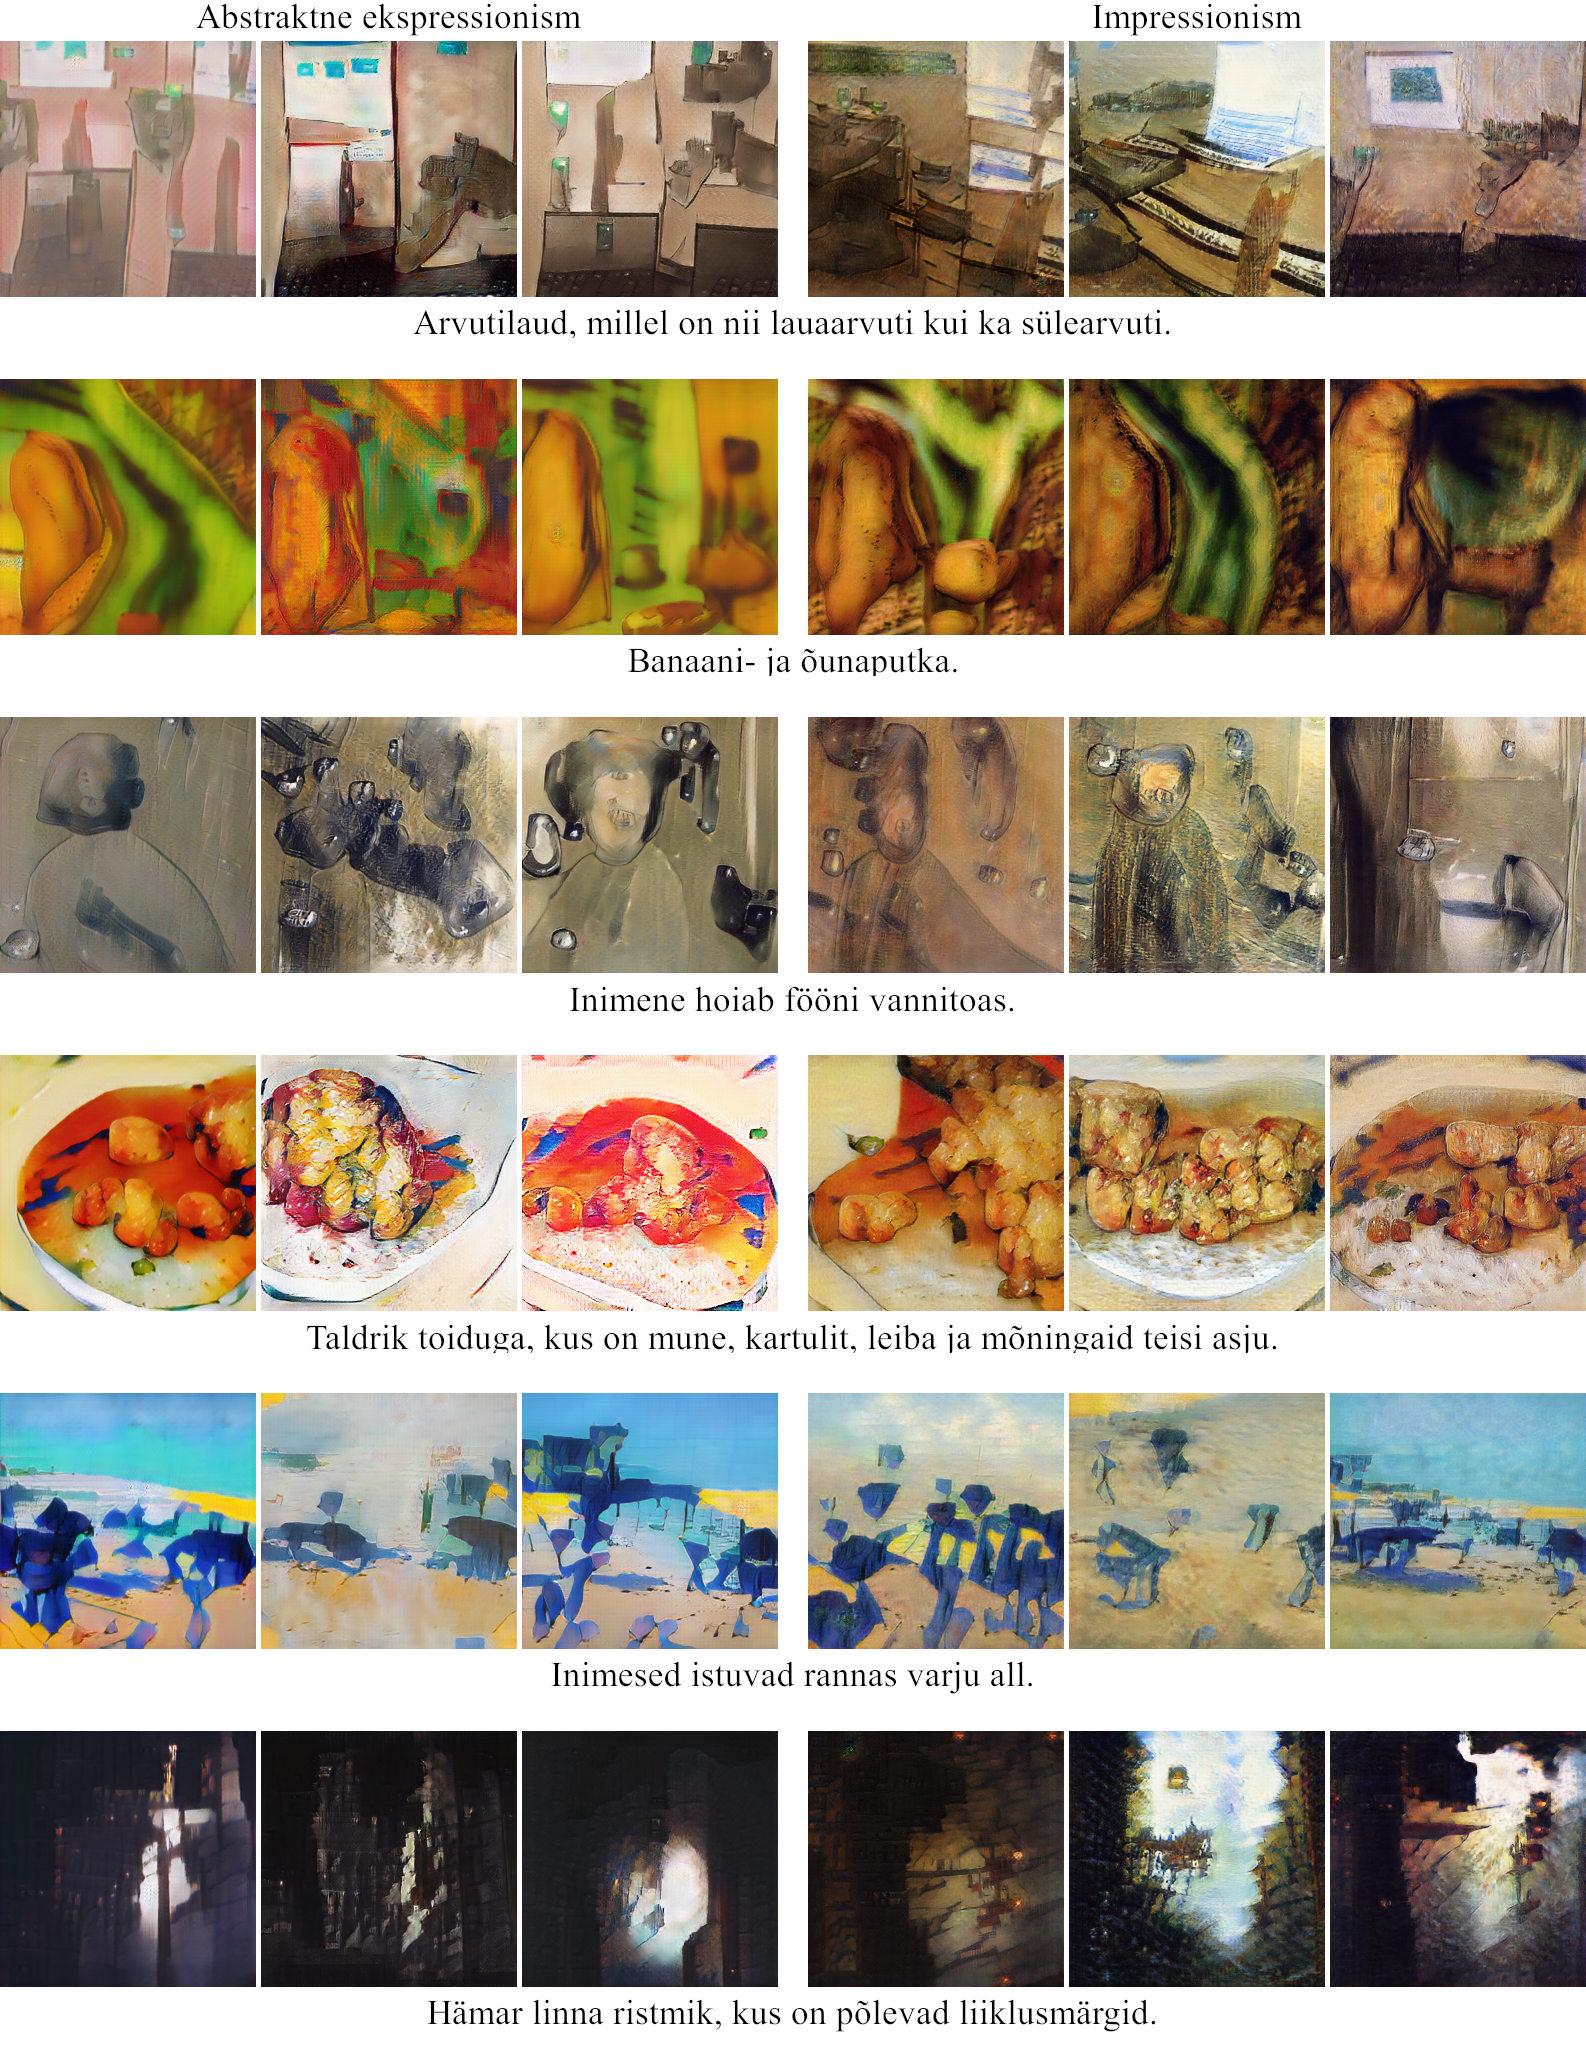
\includegraphics[width=\linewidth]{images/lisa2.png}
		\caption{Iga stiil vasakpoolse tulba puhul on CycleGAN treenitud päris piltidel ning teise kahe puhul AttnGANi poolt genereeritud pitidel; $ \lambda_{idt} = 0.5 $ esimese ja teise tulba puhul ning kolmanda tulba puhul $ \lambda_{idt} = 5 $}
		\label{fig:lisa2}
	\end{figure}

\end{document}
